% Gemini theme
% https://github.com/anishathalye/gemini

\documentclass[final]{beamer}

% ====================
% Packages
% ====================

\usepackage[T1]{fontenc}
\usepackage{lmodern}
\usepackage[size=custom,width=48,height=36,scale=0.4]{beamerposter}
\usetheme{gemini}
\usecolortheme{gemini}
\usepackage{graphicx}
\usepackage{booktabs}
\usepackage{tikz}
\usepackage{pgfplots}
\pgfplotsset{compat=1.14}
\usepackage{anyfontsize}

% ====================
% Lengths
% ====================

% If you have N columns, choose \sepwidth and \colwidth such that
% (N+1)*\sepwidth + N*\colwidth = \paperwidth
\newlength{\sepwidth}
\newlength{\colwidth}
\setlength{\sepwidth}{0.025\paperwidth}
\setlength{\colwidth}{0.3\paperwidth}

\newcommand{\separatorcolumn}{\begin{column}{\sepwidth}\end{column}}

% ====================
% Title
% ====================

\title{\centering Causal Discovery on Gut Microbial Data for Disease Risk Prediction}

\author{Mariana Paco Mendivil \inst{1} \and Candus Shi \inst{2} \and Nicole Zhang \inst{3} \and Mentor: Dr. Biwei Huang \inst{4} \and Mentor: Dr. Jelena Bradic \inst{5}}
 
\institute[shortinst]{\inst{1} mpacomendivil@ucsd.edu \samelineand \inst{2} c6shi@ucsd.edu \samelineand \inst{3} nwzhang@ucsd.edu \samelineand \inst{4} bih007@ucsd.edu \samelineand \inst{5} jbradic@ucsd.edu}

% \author{\vspace{1cm} \hspace{1cm} \raggedright Mariana Paco Mendivil \and Candus Shi \and Nicole Zhang }

% \institute {\hspace{1.6cm} \raggedright mpacomendivil@ucsd.edu \samelineand \hspace{1.2cm} c6shi@ucsd.edu \hspace{1cm} nwzhang@ucsd.edu}

% ====================
% Footer (optional)
% ====================

\footercontent{
  Please visit our website at \href{https://nzhang20.github.io/Causal-Discovery-on-Gut-Microbial-Data-for-Disease-Risk-Prediction/}{https://nzhang20.github.io/Causal-Discovery-on-Gut-Microbial-Data-for-Disease-Risk-Prediction/} or at the above QR code.}
% (can be left out to remove footer)

% ====================
% Logo (optional)
% ====================

% use this to include logos on the left and/or right side of the header:
\logoright{\includegraphics[height=1.5cm]{hdsi-white.png}}
% \logoleft{\includegraphics[height=7cm]{logo2.pdf}}

% ====================
% Body
% ====================

\begin{document}

\begin{frame}[t]
\begin{columns}[t]
\separatorcolumn

\begin{column}{\colwidth}

  \begin{block}{Background}
    \begin{itemize}
      \item \textbf{Association vs. Causation:} In many domains, researchers are often concerned with finding the underlying structure that generates the data we observe. Traditional methods make associative conclusions, but these are often insufficient to answer the scientific question. Causal discovery and causal inference are a set of methods and models that attempt to causally answer these scientific questions given the limitations of observed data \cite{pearl2016primer}.
      \item \textbf{Gut Microbiome:} The gut microbiome has been shown to be an important indicator of human health, and extensive research has been conducted to explore its impact on human health and disease. Given its diverse composition, the gut microbiome is a complex area of study as it can have heterogeneous effects for different populations \cite{baars2024gutt2d}. 
      \item \textbf{Causal Discovery and Inference in the Gut Microbiome:} Previous research has explored causal discovery in gut microbiome studies, notably using algorithms like PC-stable to construct causal networks and implement do-calculus for estimating microbe-microbe and microbe-outcome causal effects \cite{sazal2021causalgut}. More generally in the field of causal discovery, recent advancements include CD-NOD, an algorithm specifically designed for heterogeneous data, which is particularly valuable for gut microbiome research where samples often come from different studies \cite{huang2019cdnod}. 
    \end{itemize}

  \end{block}

  \begin{block}{Research Questions}

    \begin{enumerate}
      \item \textbf{Microbe-Microbe:} How do the microbe-microbe interaction networks between the healthy and diseased participants differ?
      \item \textbf{Microbe-Disease:} What microbes have a causal relationship to disease status?
      \item \textbf{Prediction:} Is it possible to predict disease status with the current composition of the dataset given causal representation learning techniques? How do they differ with the microbes learned in question 2?
    \end{enumerate}
  \end{block}

  \begin{block}{Data}

    To answer the questions above, we apply our framework to gut microbial data that investigated T2D and 
    an individual participant data meta-analysis dataset that investigated PCOS. 
    
    \begin{itemize}
      \item \textbf{T2D:} For T2D, we use the NIH Human Microbiome Project (HMP2) dataset \cite{zhou2019t2d}, filtered to healthy visits with 16S sequencing. Includes 153 insulin-sensitive (IS) and 178 insulin-resistant (IR) samples.
      \item \textbf{PCOS:} For PCOS, we use a dataset aggregated from 14 different clinical studies across Asia and Europe \cite{yang2024pcos}, filtered to individual-level samples with 16S sequencing. Includes 435 healthy controls (HC) and 513 PCOS patients.
    \end{itemize}

  \end{block}
  
	  \begin{alertblock}{Causal Discovery}
	  
	  	Causal discovery attempts to recover the true causal structure of a system given observed data. One way to model this causal structure is through a directed graphical model. A widely-used general-purpose causal discovery algorithm is the Peter-Clark (PC) algorithm \cite{glymour2019review}. It follows these key steps:
		\begin{enumerate}
		    \item Start with a \textbf{complete undirected graph} (each node connected to all other nodes).
		    \item \textbf{Remove edges} based on statistical independence and conditional independence tests.
		    \item \textbf{Identify v-structures} (patterns like $X \to Y \leftarrow Z$) to infer causal directions.
		    \item \textbf{Apply Meek’s rules} to orient additional edges while preserving v-structures.
		\end{enumerate}

	The result is a \textbf{CPDAG (Completed Partially Directed Acyclic Graph)}, which represents a set of causal structures consistent with the observed data, also known as the Markov Equivalence Class (MEC). 

	\textbf{\underline{Why Use PC?}}
			\begin{itemize}
			    \item Works for different data types (as long as independence tests match the data distribution).
			    \item Efficient for large datasets.
			    \item Assumes the \textbf{causal Markov condition}, the \textbf{faithfulness} assumption, and \textbf{no hidden confounders},.
			\end{itemize}
	  
	  \end{alertblock}

\end{column}

\separatorcolumn

\begin{column}{\colwidth}

  \begin{block}{Methods}

   In this study, we use causal discovery algorithms and compare them with 
   predictive modeling to explore the causal relationships between the 
   gut microbiome and two diseases: T2D and PCOS. Due to the high-dimensionality
   of the data and small sample sizes, we first select features through sparse
   estimation methods and sure-screening to reduce the number of microbes. 

    \begin{enumerate}
      \item \textbf{Filter out rare OTUs}. Remove microbes where all samples have less than 1\%
      relative abundance. 
      \item \textbf{Feature selection and sure screening}. For the microbe-microbe network, we use two 
      methods, SparCC \cite{friedman2012sparcc} and graphical lasso to reduce the number of edges between pairs of microbes.
      For the microbe-disease network, we use logistic lasso regression to reduce the number of 
      features that are not helpful in predicting disease. 
      \item \textbf{Causal discovery algorithms}. For the microbe-microbe network, we implement
      PC-stable with a max depth of 2. For the microbe-outcome network, we implement CD-NOD
      where the covariates correspond to the heterogeneity index. 
      \item \textbf{Variational autoencoder}. xxx. Formulas.
    \end{enumerate}

  \end{block}

  \begin{block}{T2D}

    (Report results for microbe-microbe network). From the microbe-outcome network (Figure 1), the following five genera are causal to T2D (`IRIS' node): \textit{Butyricimonas, Clostridium XIVb, Odoribacter, unclassified Bacteria,} and \textit{unclassified Firmicutes}. To further investigate their individual effects, we implement do-calculus through logistic regression models on T2D given the neighbors of the genus of interest (Table 1). We implement three models: a simple logistic regression model regressed on the five genera causal to T2D, a logistic regression model regressed on a microbe and its neighbors, and a logistic regression model regressed on a microbe and its mediators. Their significance is denoted with a \*. 

    \begin{figure}
      \centering
      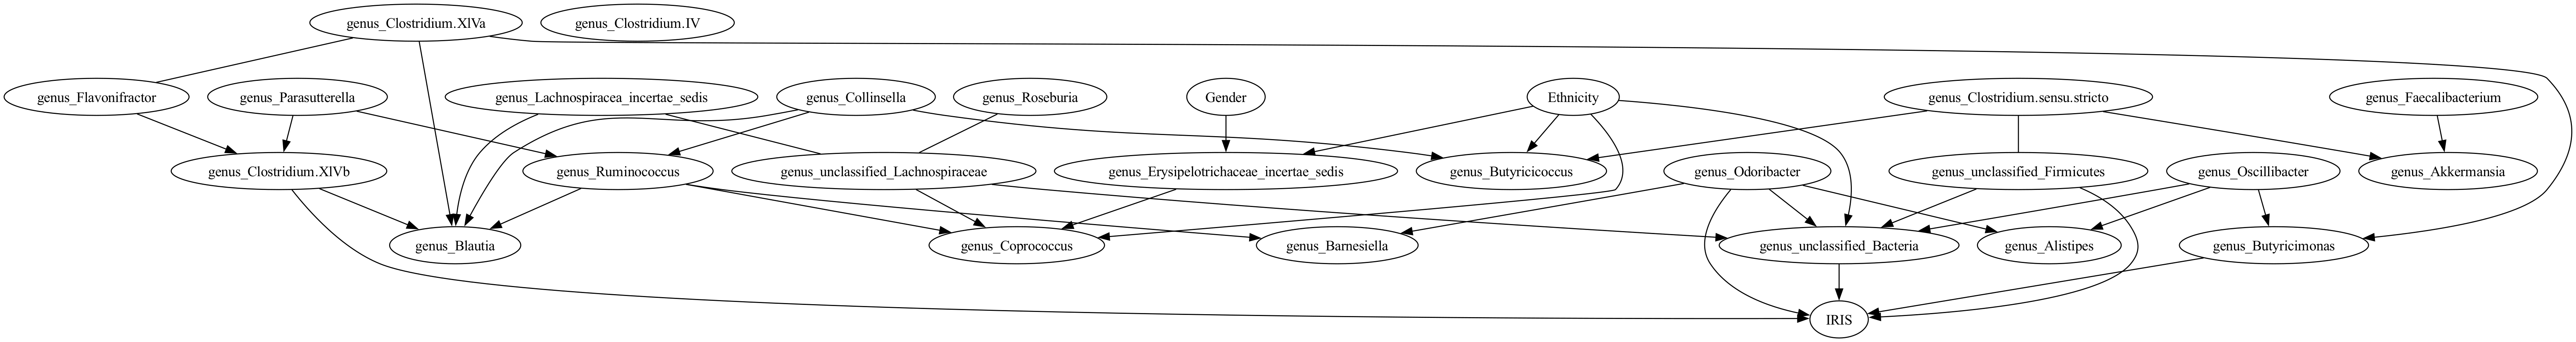
\includegraphics[width=\linewidth]{../graphs/t2d/cdnod_norm.png}
      \caption{Microbe-Disease Network for T2D.}
    \end{figure}
    
    \begin{table}
      \centering
      \begin{tabular}{l r r c}
        \toprule
        \textbf{Genus} & \textbf{Odds Ratio} & \textbf{P-Value} & \textbf{Literature Agreement} \\
        \midrule
        \textit{Butyricimonas} & 0 & 0 & Unknown \\
        \textit{Clostridium XIVb} & 0 & 0 & Unknown \\
        \textit{Odoribacter} & 0 & 0 & Unknown \\
        \textit{unclassified Bacteria} & 0 & 0 & Unknown \\
        \textit{unclassified Firmicutes} & 0 & 0 & Unknown \\
        \bottomrule
      \end{tabular}
      \caption{Do-Calculus Results for T2D.}
    \end{table}
    
    (Insert VAE results).

  \end{block}

  
\end{column}

\separatorcolumn

\begin{column}{\colwidth}

   \begin{block}{PCOS}

    (Report results for microbe-outcome network). From the microbe-outcome network (Figure 2), the following nine genera are causal to PCOS (`group' node): \textit{Alistipes, Blautia, Burkholderia, Desulfovibrio, Holdemanella, Knoellia, Prevotellaceae NK3B31 group, Ruminococcus,} and \textit{Ruminococcus gnavus group}. We find their individual causal effects with do-calculus (Table 2). 

    \begin{figure}
      \centering
      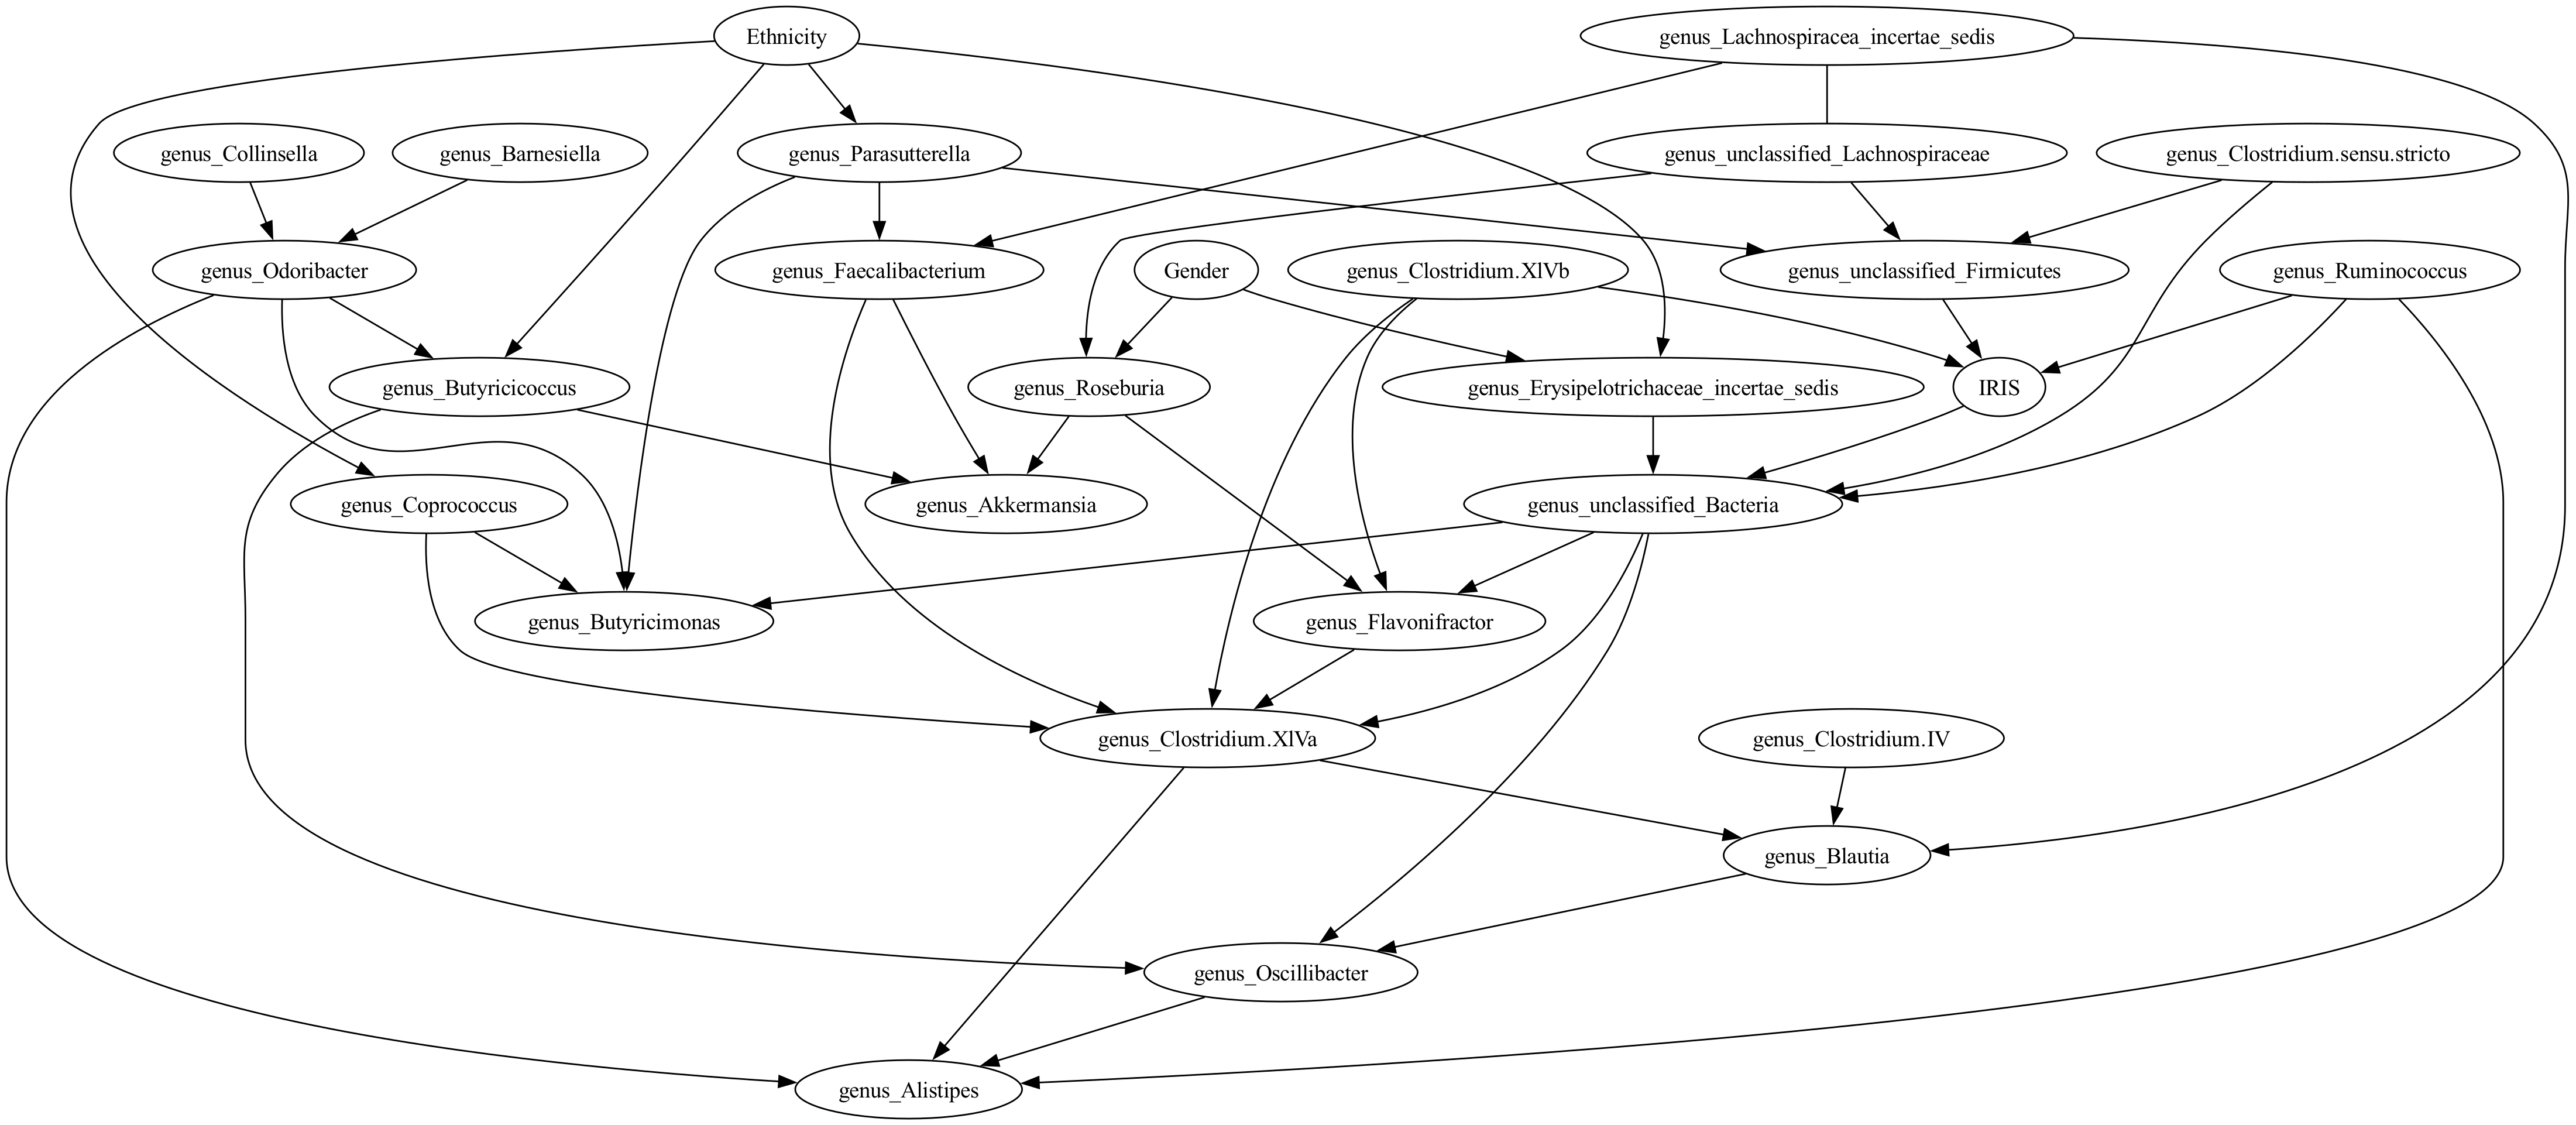
\includegraphics[width=\linewidth]{../graphs/pcos/cdnod.png}
      \caption{Microbe-Disease Network for PCOS.}
    \end{figure}
    
    \begin{table}
      \centering
      \begin{tabular}{l r r c}
        \toprule
        \textbf{Genus} & \textbf{Model 1} & \textbf{Model 2} & \textbf{Literature Agreement} \\
        \midrule
        \textit{Alistipes} & 0.153458 & 4.68e-05 & Unknown \\
        \textit{Blautia} & 0 & 0 & Unknown \\
        \textit{Burkholderia} & 0 & 0 & Unknown \\
        \textit{Desulfovibrio} & 0 & 0 & Unknown \\
        \textit{Holdemanella} & 0 & 0 & Unknown \\
        \textit{Knoellia} & 0 & 0 & Unknown \\
        \textit{Prevotellaceae NK3B31 group} & 0 & 0 & Unknown \\
        \textit{Ruminococcus} & 0 & 0 & Unknown \\
        \textit{Ruminococcus gnavus group} & 0 & 0 & Unknown \\
        \bottomrule
      \end{tabular}
      \caption{Do-Calculus Results for PCOS.}
    \end{table}

   (Insert VAE results).

  \end{block}

  \begin{block}{Conclusion \& Future Work}

    Answer questions 1, 2, and 3. Explain BIRDMAn. Point to website for more results. Fix references to et al for many authors. We would like to thank our mentors and Dr. Sam Degregori for guidance throughout this project. 
    
  \end{block}

  \begin{block}{References}

    \footnotesize{\bibliographystyle{unsrt}\bibliography{../report/reference}}

  \end{block}

\end{column}

\separatorcolumn
\end{columns}
\end{frame}

\end{document}